\documentclass[oneside,a4paper,14pt]{extarticle}
\usepackage[a4paper,letterpaper,top=20mm,bottom=20mm,left=20mm,right=10mm]{geometry}
\usepackage[russian]{babel}
\usepackage{indentfirst}
\usepackage{amsmath}
\usepackage{amsfonts}
\usepackage{amsthm}
\usepackage{graphicx}
\usepackage{caption}
\usepackage{titlesec}
\usepackage{minted, fancyvrb}

\titleformat{\section} {\normalsize\bfseries} {\thesection} {1em} {}
\titleformat{\subsection} {\normalsize\bfseries} {\thesubsection} {1em} {}
\titleformat{\subsubsection} {\normalsize\bfseries} {\thesubsection} {1em} {}
\renewcommand\baselinestretch{1.45}\normalsize
\setlength{\parindent}{1.25cm}

\begin{document}

\newpage
\thispagestyle{empty}
\begin{center}
	МИНИСТЕРСТВО НАУКИ И ВЫСШЕГО ОБРАЗОВАНИЯ РОССИЙСКОЙ ФЕДЕРАЦИИ ФЕДЕРАЛЬНОЕ ГОСУДАРСТВЕННОЕ БЮДЖЕТНОЕ ОБРАЗОВАТЕЛЬНОЕ УЧРЕЖДЕНИЕ ВЫСШЕГО ОБРАЗОВАНИЯ\\
	«ВЯТСКИЙ ГОСУДАРСТВЕННЫЙ УНИВЕРСИТЕТ»\\
	Институт математики и информационных систем\\
	Факультет автоматики и вычислительной техники\\
	Кафедра электронных вычислительных машин
\end{center}
\vspace{10mm}

\hfill
\begin{tabular}{l}
  \footnotesize Дата сдачи на проверку: \\
  \footnotesize <<\rule[-1mm]{5mm}{0.10mm}\/>>\rule[-1mm]{20mm}{0.10mm}\ 2025 г.\\
  \footnotesize Проверено: \\
  \footnotesize <<\rule[-1mm]{5mm}{0.10mm}\/>>\rule[-1mm]{20mm}{0.10mm}\ 2025 г. \\
\end{tabular}
\vfill

\begin{center}
    ПРЕДСТАВЛЕНИЕ ГРАФИКОВ. МАТРИЦА ИНЦИДЕНТНОСТИ.\\
	Отчёт по лабораторной работе №3\\
	по дисциплине\\
	<<Дискретная математика>>\\
\end{center}
\vspace{25mm}
\noindent
\begin{tabular}{ll}
	Разработал студент гр. ИВТб-1301-05-00 & \rule[-1mm]{30mm}{0.10mm}\,/Черкасов А. А./   \\
	                                       & \hspace{8mm}\footnotesize(подпись)            \\
	Проверила преподаватель                & \rule[-1mm]{30mm}{0.10mm}\,/Пахарева И. В./ \\
	                                       & \hspace{8mm}\footnotesize(подпись)            \\
\end{tabular}

\noindent
  \begin{tabular}{lp{58mm}r}
    Работа защищена &  & <<\rule[-1mm]{5mm}{0.10mm}\/>>\rule[-1mm]{30mm}{0.10mm}\ 2025 г.
  \end{tabular}
  \vfill

\begin{center}
	Киров\\
	2025
\end{center}

\newpage\thispagestyle{plain}

\section*{Цель}

Цель работы: изучение представления ориентированных графов в виде матрицы инцидентности и алгоритмический анализ этой структуры для поиска двунаправленных дуг.

\section*{Задание}
\begin{itemize}
	\item[$-$] По матрице инцидентности, заданной в файле \texttt{input.txt}, определить количество двунаправленных дуг графа.
	\item[$-$] Вывести множество найденных дуг (по номерам вершин), то есть пары вершин, между которыми имеются ребра в обоих направлениях.
\end{itemize}
\section*{Решение}

Схема алгоритма решения представлена на рисунке 1. Пример работы программы представлен на рисунках 2.1 и 2.2. Исходный код решений представлен в Приложениях A1, A2 и A3.

\clearpage
\begin{figure}[H]
	\centering
	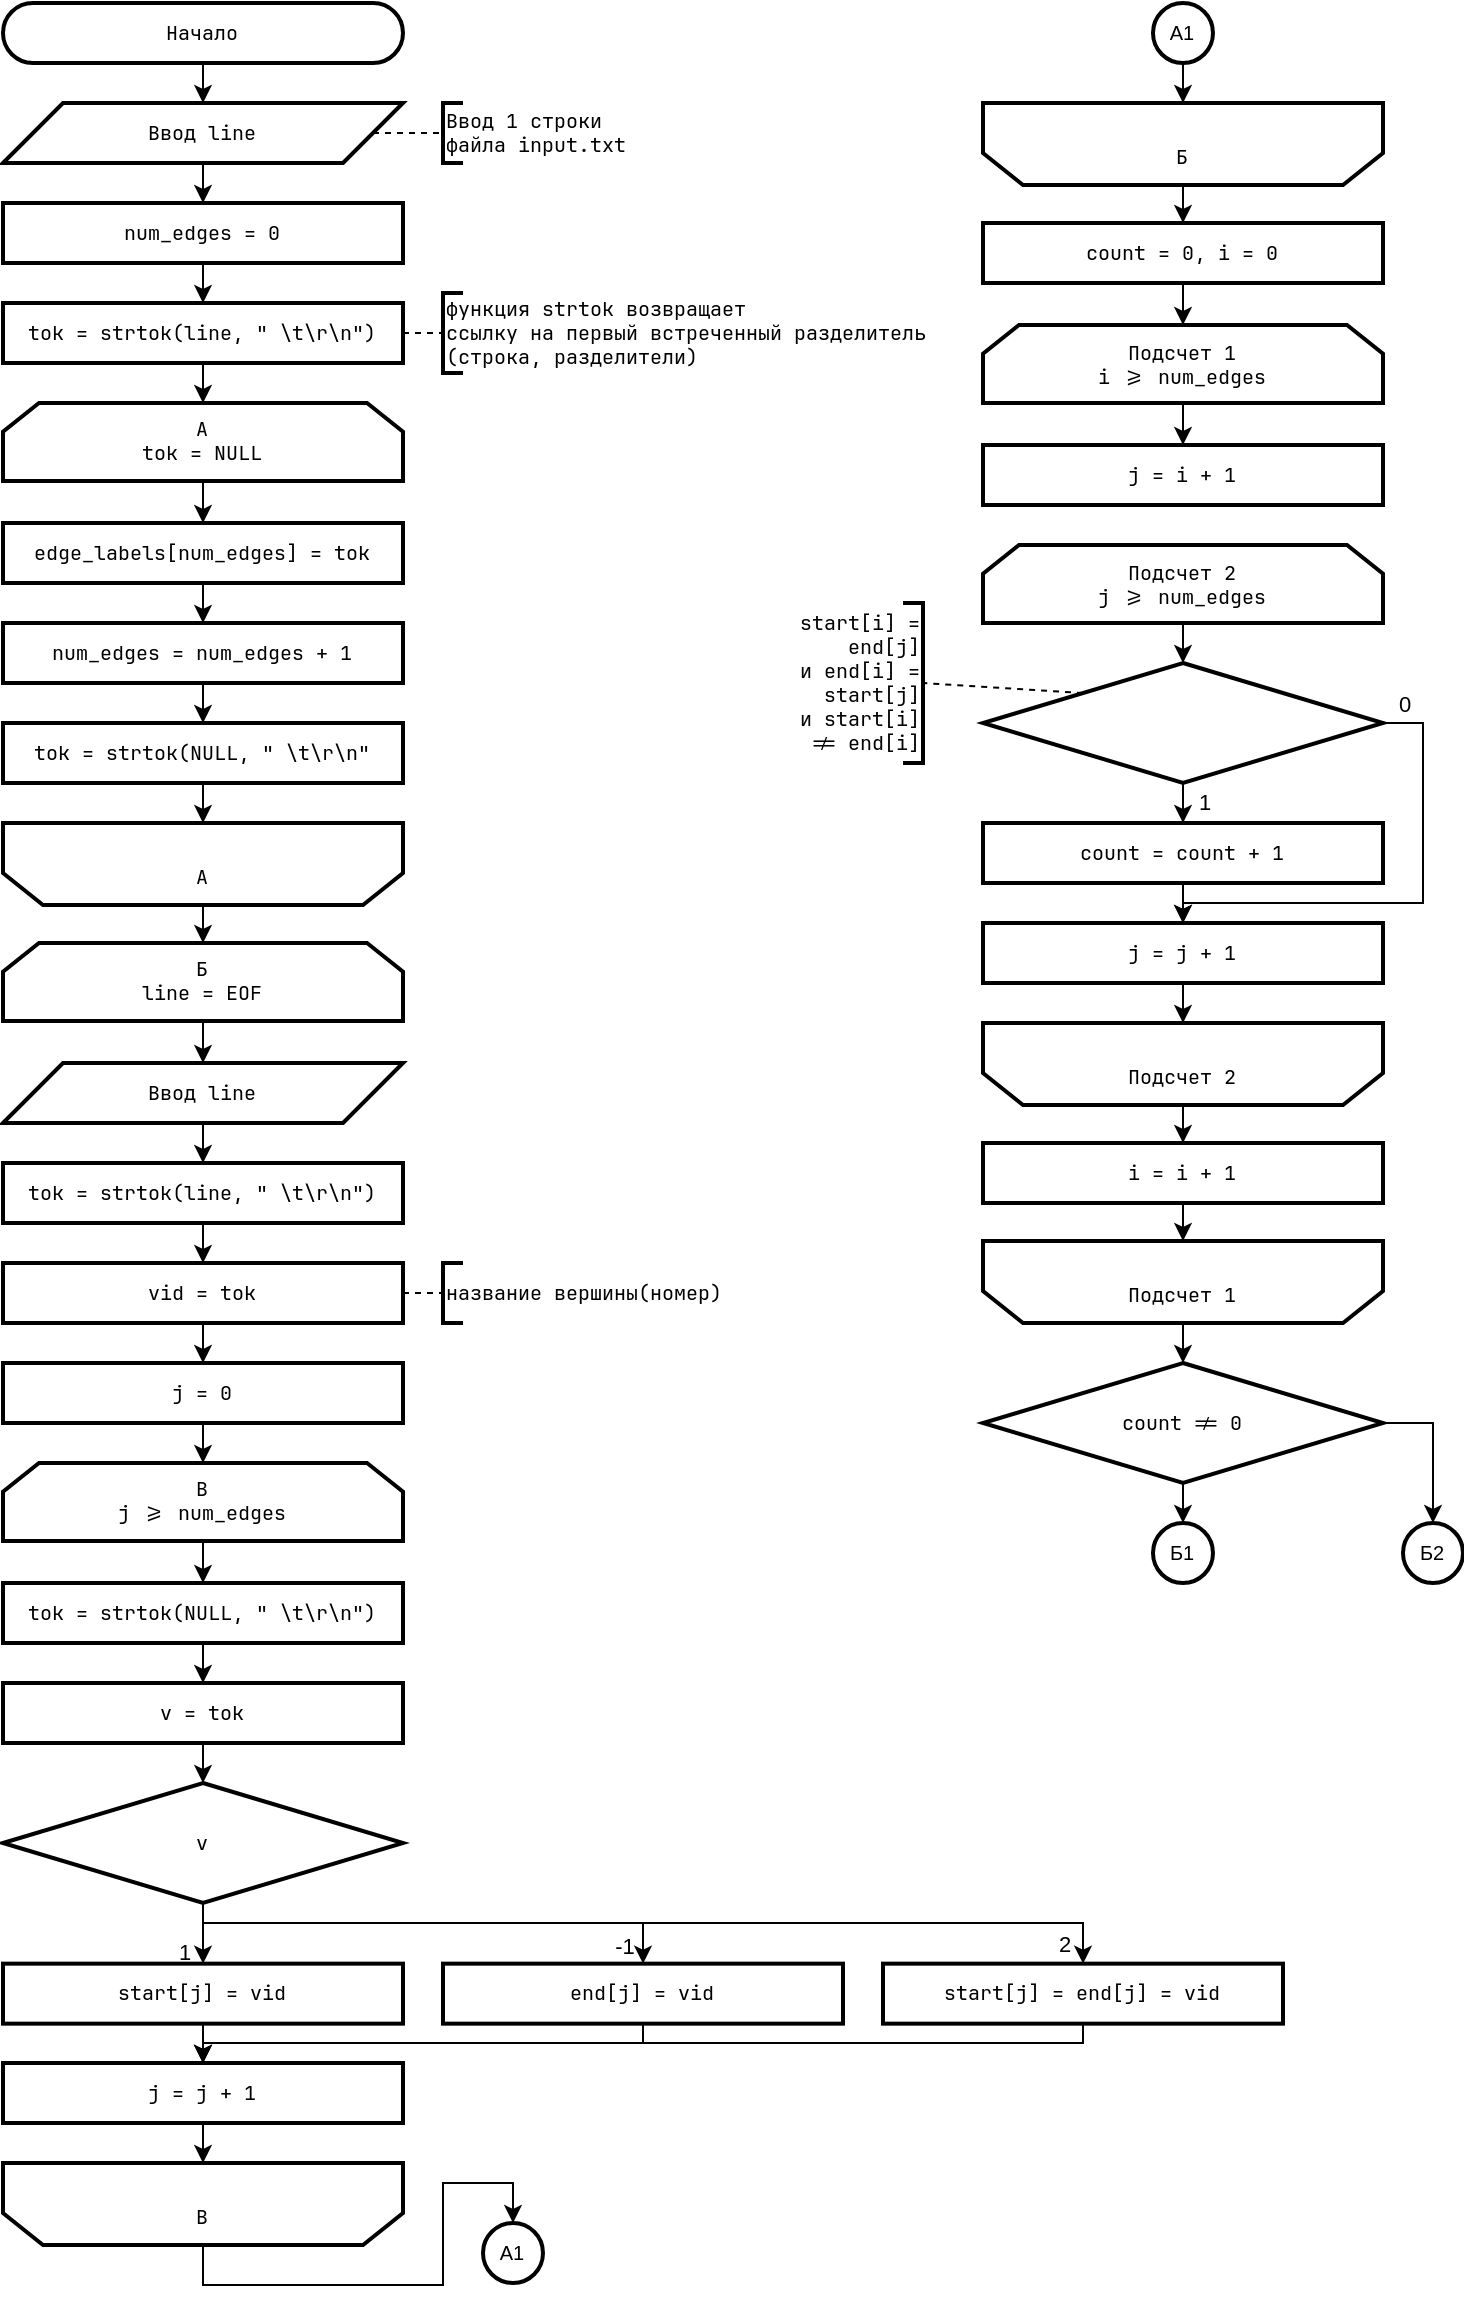
\includegraphics[height=0.9\textheight]{pics/flowchart1.png}
	\caption*{Рисунок 1.1 - Схема алгоритма основной программы стр.1.}
\end{figure}

\clearpage
\begin{figure}[H]
	\centering
	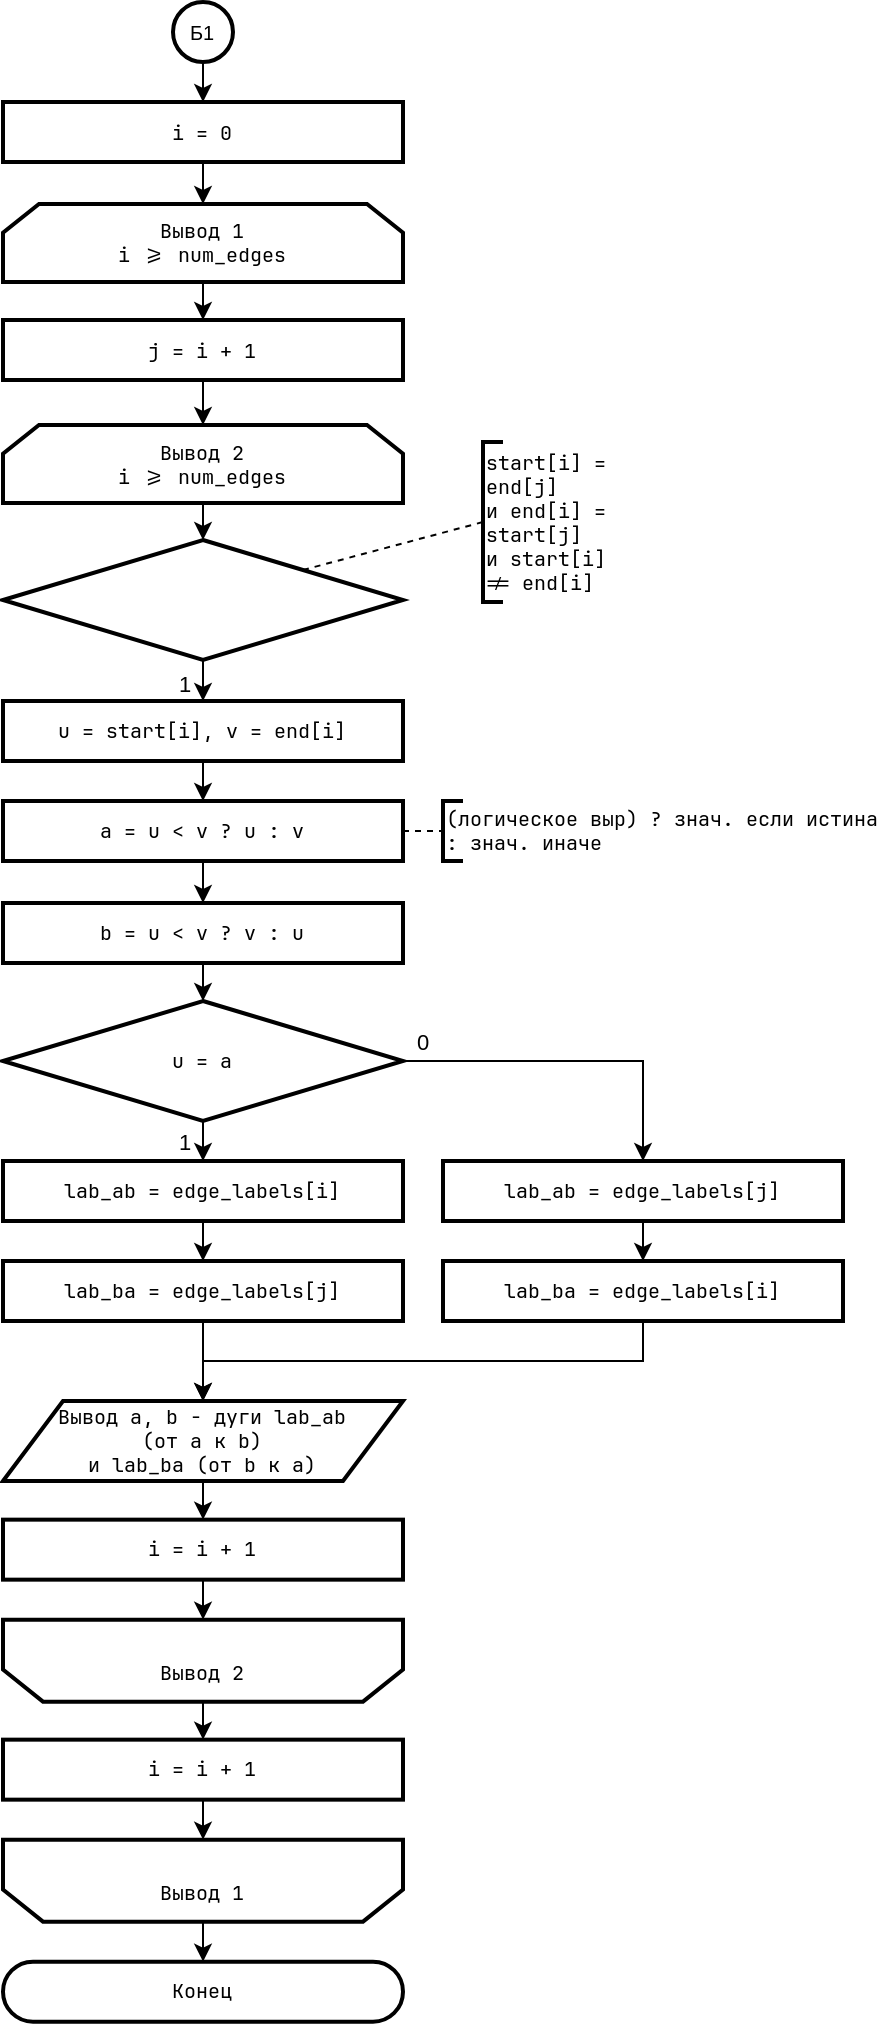
\includegraphics[height=0.9\textheight]{pics/flowchart2.png}
	\caption*{Рисунок 1.2 - Схема алгоритма основной программы стр.2.}
\end{figure}

\clearpage
\begin{figure}[H]
	\centering
	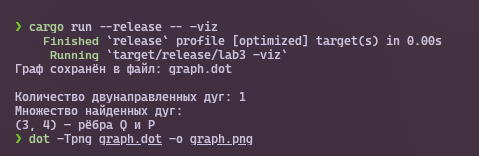
\includegraphics[width=0.9\textwidth]{pics/screen.png}
	\caption*{Рисунок 2.1 - Пример работы программы.}
\end{figure}

\begin{figure}[H]
	\centering
	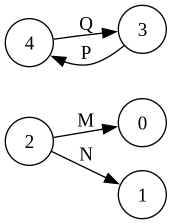
\includegraphics[height=0.5\textheight]{pics/graph.png}
	\caption*{Рисунок 2.2 - Сгенерированный по входному файлу input.txt граф.}
\end{figure}

\section*{Вывод}

\setminted{style = rainbow_dash, fontsize = \small} % https://pygments.org/styles/

В ходе выполнения данной лабораторной работы была разработана и отлажена программа на языке Rust, которая:
\begin{itemize}
    \item Считывает матрицу инцидентности из текстового файла \texttt{input.txt}.
    \item Корректно разбирает каждый столбец-метку для выявления начальной и конечной вершины дуги.
    \item Определяет двунаправленные дуги (пары вершин, между которыми существуют дуги в обоих направлениях), исключая петли и одинаковые метки.
    \item Выводит количество таких двунаправленных дуг и подробную информацию о каждом ребре (номера вершин и соответствующие метки).
\end{itemize}

\newpage
\section*{Приложение А1. Исходный код}
\inputminted{rust}{src/main.rs}

\newpage
\section*{Приложение А2. Исходный код}
\inputminted{rust}{src/graphviz.rs}

\newpage
\section*{Приложение А3. Входной файл.}
\inputminted{text}{./input.txt}

\end{document}
